\begin{frame}{Deterministic Deep Neural Networks for Solving PDEs}

\textbf{Main ideas}:
\begin{itemize}
%\item We approximate the PDE solution by a Deep Neural Network (DNN):
%\begin{equation*}
%u \approx u_{NN}.
%\end{equation*}

\item We select a loss function $\mathcal{L}_{(\cdot)}$ whose minimizer solves the PDE.

\item We train the DNN:
\begin{equation*}
u_{NN,\theta^*} := \underset{u_{NN,\theta}, \theta \in \Theta}{\textup{ arg min }} \mathcal{L}(u_{NN,\theta}).
\end{equation*}

\end{itemize}


\textbf{Key ingredients:}
\begin{itemize}
\item Build a DNN architecture $u_{NN,\theta}$.
\item Define the loss function  $\mathcal{L}(u_{NN,\theta})$.
\item Select a quadrature rule to numerically evaluate $\mathcal{L}(u_{NN,\theta})$.
\item Choose minimization algorithm (SGD, Adam, RMSprop...).
\end{itemize}
\end{frame}
%%%%%%%%%%%%%%%%%%%%%%%%%%%%%%%%%%%%%%%%%%%%%%%%%%%%%%%%%%%%%%%%%%%%%%%
%%%%%%%%%%%%%%%%%%%%%%%%%%%%%%%%%%%%%%%%%%%%%%%%%%%%%%%%%%%%%%%%%%%%%%%
%%%%%%%%%%%%%%%%%%%%%%%%%%%%%%%%%%%%%%%%%%%%%%%%%%%%%%%%%%%%%%%%%%%%%%%

\begin{frame}{Architecture Sketch}
\def\layersep{1.5cm}
\centering

%\begin{tikzpicture}[x=1cm,y=0.8cm]
%%\draw[very thin, rounded corners=5pt,fill=orange!30!white ,opacity=0.5] (4.0,0.2) rectangle (10,1.3);
%\node at (7.0,0.75){\Large $u \approx u_{NN} := \underset{\theta \in V}{\textup{ arg min }} \mathcal{L}_{(\cdot)}(\theta)$};
%\end{tikzpicture}
%
%\vspace{0.4cm}

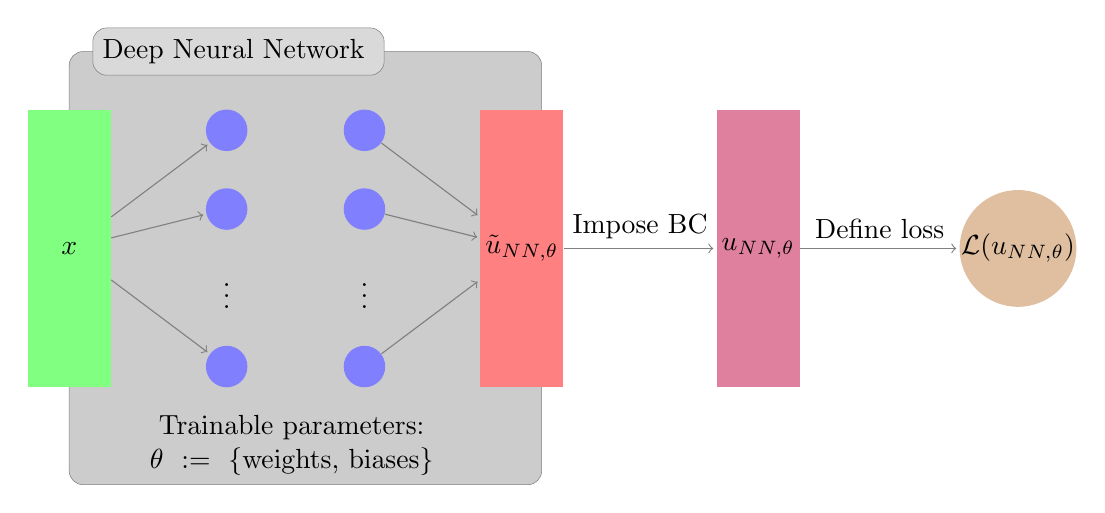
\begin{tikzpicture}[shorten >=1pt,->,draw=black!50, node distance=\layersep]
    \tikzstyle{every pin edge}=[<-,shorten <=1pt]
    \tikzstyle{neuron}=[circle,fill=black!25,minimum size=20pt,inner sep=0pt]
    \tikzstyle{neuron2}=[circle,fill=black!25,minimum size=15pt,inner sep=0pt]
    \tikzstyle{input lay}=[rectangle,fill=green!50,minimum width=30pt, minimum height=100pt,inner sep=0pt]
%    \tikzstyle{input neuron}=[neuron, fill=green!50];
	\tikzstyle{hidden neuron}=[neuron2, fill=blue!50];
	\tikzstyle{ghost neuron}=[neuron, fill=gray!40!white, , opacity=1];
    \tikzstyle{output neuron}=[neuron, fill=red!50];
    \tikzstyle{output lay}=[rectangle,fill=red!50,minimum width=30pt, minimum height=100pt,inner sep=0pt]
    
	\tikzstyle{multi neuron}=[neuron, fill=purple!50];
    \tikzstyle{multi lay}=[rectangle,fill=purple!50,minimum width=30pt, minimum height=100pt,inner sep=0pt]	
	
	
	\tikzstyle{final neuron}=[neuron, fill=brown!50];
	
    \tikzstyle{annot} = [text width=4em, text centered]
	\tikzstyle{annot final} = [text width=10em, text centered]


\draw[very thin, rounded corners=5pt,fill=gray!40!white ,opacity=1] (0,1.5) rectangle (6,-4);
\draw[very thin, rounded corners=5pt,fill=gray!30!white ,opacity=1] (0.3,1.8) rectangle (4.0,1.2);
\node [anchor = west] at (0.3,1.5){Deep Neural Network};

    % Draw the input layer nodes
    \foreach \name / \y in {1}
        \node[input lay] (I-\name) at (0,-1) {$x$};

%    % Draw the hidden layer nodes
%    \foreach \name / \y in {1,...,3}
%        \path[yshift=1.5cm]
%            node[hidden neuron, xshift=0.5cm] (H-\name) at (\layersep,-\y cm) {};
	
\path[yshift=1.5cm] node[hidden neuron, xshift=0.5cm] (H1_1) at (\layersep,-1 cm) {};	
\path[yshift=1.5cm] node[hidden neuron, xshift=0.5cm] (H1_2) at (\layersep,-2 cm) {};
\path[yshift=1.5cm] node[ghost neuron, xshift=0.5cm] (Hghost1) at (\layersep,-3 cm) {$\vdots$};
\path[yshift=1.5cm] node[hidden neuron, xshift=0.5cm] (H1_3) at (\layersep,-4 cm) {};
	
\path[yshift=1.5cm] node[hidden neuron, xshift=0.0cm] (H2_1) at (2.5*\layersep,-1 cm) {};	
\path[yshift=1.5cm] node[hidden neuron, xshift=0.0cm] (H2_2) at (2.5*\layersep,-2 cm) {};
\path[yshift=1.5cm] node[ghost neuron, xshift=0.0cm] (Hghost2) at (2.5*\layersep,-3 cm) {$\vdots$};
\path[yshift=1.5cm] node[hidden neuron, xshift=0.0cm] (H2_3) at (2.5*\layersep,-4 cm) {};

\path[yshift=1.5cm] node[ghost neuron, xshift=0.2cm] (Hghosta) at (1.75*\layersep,-1 cm) {$\hdots$};
\path[yshift=1.5cm] node[ghost neuron, xshift=0.2cm] (Hghostb) at (1.75*\layersep,-2 cm) {$\hdots$};
\path[yshift=1.5cm] node[ghost neuron, xshift=0.2cm] (Hghostc) at (1.75*\layersep,-4 cm) {$\hdots$};

%    % Draw the output layer node
    \node[output lay, right of=Hghost2, yshift=0.5cm, xshift=0.5cm] (O) {$\tilde{u}_{NN, \theta}$};
    
    % Multiply BC function
	\node[multi lay, right of=O,  xshift=1.5cm] (M) {$u_{NN, \theta}$};
%	\node[multi lay, right of=Hghost2, yshift=0.5cm, xshift=0.5cm] (M) {$u_{NN}$};
	
	% Final output, after Loss
	\node[final neuron, right of=M, xshift=1.8cm] (F) {$\mathcal{L}(u_{NN, \theta})$};

    % Connect every node in the input layer with every node in the
    % hidden layer.
    \foreach \source in {1}
        \foreach \dest in {1,...,3}
            \path (I-\source) edge (H1_\dest);

    % Connect every node in the hidden layer with the output layer
    \foreach \source in {1,...,3}
        \path (H2_\source) edge (O);
        
%	% Connect output kayer and multiply layer
	\path[every node/.style={anchor=south}] (O) edge node {Impose BC} (M);
	
	% Connect output kayer and multiply layer
	\path[every node/.style={anchor=south}] (M) edge node {Define loss} (F);

    % Annotate the layers
%    \node[text width=10em, text centered, ,above of=Hghosta, node distance=0.7cm] {Hidden layers};
    \node (texto)[text width=15.5em, text centered, ,below of=Hghostc, node distance=1cm] {Trainable parameters: \\ $\theta:= \{$weights, biases$\}$};
    
%    \node[text width=6.5em, text centered, ,right of=texto, node distance=4.5cm] {Non-trainable layer};
%    \node[text width=6.5em, text centered, ,right of=texto, node distance=7.5cm] {Non-trainable layer};
    
%    \node[text width=4em, text centered, ,above of=I-1, node distance=2.cm] {\footnotesize INPUT};
%    \node[text width=4em, text centered, ,above of=F, node distance=1.cm] {\footnotesize OUTPUT};
\end{tikzpicture}

\vspace{0.2cm}
\small To impose the homogeneous Dirichlet BC, we define:

$u_{NN, \theta} := \phi(x) \cdot \tilde{u}_{NN, \theta}$, where 
$ \left\{
\begin{array}{l}
\phi(x) = 0,  \quad \text{if} \; x \in \Gamma_D,\\ 
\phi(x) \neq 0, \quad \text{if} \; x \not \in \Gamma_D.
\end{array}
\right.$

\end{frame}
%%%%%%%%%%%%%%%%%%%%%%%%%%%%%%%%%%%%%%%%%%%%%%%%%%%%%%%%%%%%%%%%%%%